\documentclass[11pt]{article}
\input{../../notes-style.tex}

\title{CS 300 -- Chapter 7 Notes\\\large Heaps and Priority Queues}
\author{Jose de Lima}
\date{\today}

\begin{document}
\maketitle

\section{7.1 Heaps: The Big Idea}

A \textbf{heap} is a binary tree specialized for one job: hand me the max (or min) element, fast, and let me insert or remove in logarithmic time. It is not a BST -- it deliberately gives up ordered iteration to gain simplicity and speed on that narrow interface. Where a BST balances every subtree to permit arbitrary search, a heap only cares that \emph{the root is the extremum}.

\begin{defnbox}[Max-heap property]
A binary tree satisfies the \emph{max-heap property} if, for every node $n$:
\[
n.\text{key} \;\ge\; n.\text{left}.\text{key}
\quad \text{and} \quad
n.\text{key} \;\ge\; n.\text{right}.\text{key}
\]
(where absent children are ignored). By transitivity, the root's key is $\ge$ every descendant -- \emph{the root holds the maximum}.
\end{defnbox}

The \textbf{min-heap} is the mirror image: swap $\ge$ for $\le$. The root holds the minimum. Everything we say about max-heaps inverts cleanly.

\subsection*{What a heap is \emph{not}}

\begin{warnbox}
A heap is \textbf{not} a BST. The left and right subtrees are not sorted relative to each other -- only relative to their parent. You cannot in-order traverse a heap and get sorted output. You cannot binary-search a heap for an arbitrary key. A heap is optimized for \emph{extremum access}, nothing else.
\end{warnbox}

A quick check: in the BST from chapter 6, \texttt{node->left < node < node->right}. In a max-heap, \texttt{node->left $\le$ node} and \texttt{node->right $\le$ node}, but \texttt{node->left} and \texttt{node->right} are unordered with respect to each other. Two completely different invariants.

\subsection*{Why not just use a sorted list?}

We already have structures that hand over the max in $O(1)$:
\begin{itemize}[leftmargin=*]
    \item A sorted array: max is at the last index. Remove: $O(1)$. Insert: $O(n)$ to find the spot and shift.
    \item A BST: max is at the rightmost node. Insert/remove: $O(h) = O(\log n)$ balanced, $O(n)$ skewed.
    \item A sorted linked list: max at the tail. Insert: $O(n)$.
\end{itemize}

A heap beats all of these for the ``give me the max, keep handing me max, occasionally insert new stuff'' workload:

\begin{center}
\begin{tabular}{lllll}
Structure & Peek max & Remove max & Insert & Notes \\
\hline
Sorted array         & $O(1)$ & $O(1)$      & $O(n)$ & shifts on insert \\
Sorted linked list   & $O(1)$ & $O(1)$      & $O(n)$ & scan on insert \\
Unsorted array       & $O(n)$ & $O(n)$      & $O(1)$ & rescan per op \\
Balanced BST         & $O(\log n)$ & $O(\log n)$ & $O(\log n)$ & overkill \\
\textbf{Max-heap}    & $\mathbf{O(1)}$ & $\mathbf{O(\log n)}$ & $\mathbf{O(\log n)}$ & perfect fit \\
\end{tabular}
\end{center}

The heap trades away ordered iteration and arbitrary search (which we don't need for this workload) to get $O(\log n)$ insert with $O(1)$ peek.

\subsection*{The canonical use case: priority queues}

A \textbf{priority queue} is an abstract data type that supports \texttt{insert(item, priority)}, \texttt{extractMax()} (or \texttt{extractMin()}), and \texttt{peek()}. Heaps are the standard implementation. Real-world examples:

\begin{itemize}[leftmargin=*]
    \item \textbf{OS process schedulers:} ready processes live in a max-heap keyed by priority; the scheduler extracts the highest-priority ready process on each quantum.
    \item \textbf{Online support queues:} customers live in a min-heap keyed by ``order of arrival + urgency bonus'' -- whoever has the lowest number (highest effective priority) gets the next agent. This is a common running example in textbooks.
    \item \textbf{Dijkstra / A* / Prim:} graph algorithms repeatedly extract the next ``cheapest'' frontier node. A min-heap makes those $O((V+E) \log V)$.
    \item \textbf{Event simulations:} an event-loop heap keyed by simulated timestamp lets you pop ``next event'' efficiently.
    \item \textbf{Top-$k$ queries:} maintain a min-heap of size $k$; for each incoming item, if it's bigger than the heap's min, pop and push. Net $O(n \log k)$ instead of $O(n \log n)$ for ``top 10 from a stream of a million.''
\end{itemize}

\subsection*{The two core operations}

Every heap algorithm reduces to two primitives. In a max-heap:

\begin{defnbox}[Percolate up / Percolate down]
\textbf{Percolate up} (also ``bubble up'' or ``sift up''): take a node whose key might be too large for its parent. While the node's key $>$ its parent's key, swap with parent. Used after insertion.

\textbf{Percolate down} (``bubble down'' / ``sift down''): take a node whose key might be too small for its children. While the node has a child with a larger key, swap with the larger child. Used after the root is removed.
\end{defnbox}

Both run in $O(\log n)$ because the tree is kept \textbf{complete} -- every level is full except possibly the last, which fills left-to-right. Completeness forces height $= \lfloor \log_2 n \rfloor$, so a single root-to-leaf path is logarithmic.

\subsection*{Insert: percolate up}

\begin{enumerate}[leftmargin=*]
    \item Place the new node in the next available slot (leftmost position on the deepest level, extending to a new level if the current one is full). This preserves completeness.
    \item Compare the new node to its parent. If it's larger, swap. Repeat until the parent is larger or we reach the root.
\end{enumerate}

Walk-through: insert $42$ into

\begin{center}
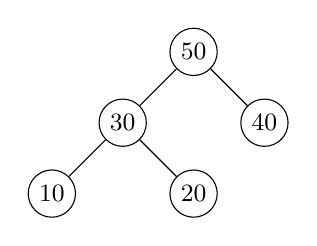
\begin{tikzpicture}[level distance=9mm, sibling distance=18mm,
    every node/.style={circle, draw, minimum size=6mm, inner sep=0pt, font=\small}]
    \node {50}
        child {node {30} child {node {10}} child {node {20}}}
        child {node {40}};
\end{tikzpicture}
\end{center}

Step 1: attach $42$ as right child of $40$ (first empty slot):

\begin{center}
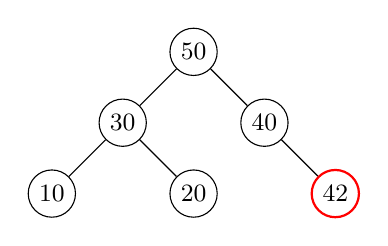
\begin{tikzpicture}[level distance=9mm, sibling distance=18mm,
    every node/.style={circle, draw, minimum size=6mm, inner sep=0pt, font=\small}]
    \node {50}
        child {node {30} child {node {10}} child {node {20}}}
        child {node {40} child[missing] {} child {node[draw=red, thick] {42}}};
\end{tikzpicture}
\end{center}

Step 2: $42 > 40$? Yes. Swap.

\begin{center}
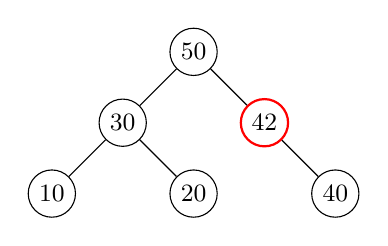
\begin{tikzpicture}[level distance=9mm, sibling distance=18mm,
    every node/.style={circle, draw, minimum size=6mm, inner sep=0pt, font=\small}]
    \node {50}
        child {node {30} child {node {10}} child {node {20}}}
        child {node[draw=red, thick] {42} child[missing] {} child {node {40}}};
\end{tikzpicture}
\end{center}

Step 3: $42 > 50$? No. Stop. Heap property restored.

\subsection*{Remove (max): replace-and-percolate-down}

\begin{enumerate}[leftmargin=*]
    \item Save the root's value (that's the answer we return).
    \item Take the \emph{last} node (rightmost leaf of the deepest level) and put it at the root. Delete the now-duplicate last slot. This preserves completeness but usually breaks the heap property at the root.
    \item Percolate down: compare the new root against its two children. If the larger child is greater than the node, swap with that child. Repeat until no larger child exists or the node reaches a leaf.
\end{enumerate}

The ``replace with last then percolate down'' dance is the whole algorithm. You're not finding a replacement by careful search -- you grab the structural last node to keep the tree complete, and then let percolate-down sort out the resulting local violation.

\begin{ideabox}
Heaps are the cleanest example in this course of \emph{trading generality for speed}. They give up ordered search, in-order traversal, and range queries -- capabilities a BST provides -- to get a guaranteed $O(1)$ peek and $O(\log n)$ insert/extract with a tiny implementation. Whenever you only need the extremum (and not ordered iteration), reach for a heap first.
\end{ideabox}

\subsection*{In the C++ STL}

\texttt{std::priority\_queue} is a max-heap by default, built on top of \texttt{std::vector}:

\begin{lstlisting}
#include <queue>
std::priority_queue<int> pq;        // max-heap of ints
pq.push(30); pq.push(50); pq.push(40);
std::cout << pq.top();              // 50
pq.pop();
std::cout << pq.top();              // 40
\end{lstlisting}

For a min-heap, pass \texttt{std::greater}:

\begin{lstlisting}
std::priority_queue<int, std::vector<int>, std::greater<int>> minpq;
\end{lstlisting}

Section 7.2 will show how the tree is actually stored -- surprise, not with pointers. Sections 7.3 and 7.4 formalize \texttt{percolateUp} and \texttt{percolateDown}. Section 7.5 builds the priority-queue ADT on top.

\section{7.2 Heaps Stored in Arrays}

Here's the twist: the binary tree in chapter 6 uses a \texttt{TreeNode} struct with \texttt{left}, \texttt{right}, (\texttt{parent}) pointers per node. A heap uses \textbf{nothing of the sort.} A heap is almost always stored as a plain array, with all parent/child relationships computed by \emph{index arithmetic}. No pointers, no allocations per node, no cache misses on node traversal. This is the single biggest reason the heap is the go-to priority queue in practice.

\begin{defnbox}[Array representation of a complete binary tree]
Number the nodes level by level, left to right, starting from the root at index 0. For a node at index $i$:
\[
\text{parent}(i) = \left\lfloor \frac{i-1}{2} \right\rfloor
\qquad
\text{leftChild}(i) = 2i + 1
\qquad
\text{rightChild}(i) = 2i + 2
\]
These formulas require the tree to be \emph{complete} -- every level full except possibly the last, which fills left-to-right. That's exactly the property heap operations preserve.
\end{defnbox}

\subsection*{Example}

\begin{center}
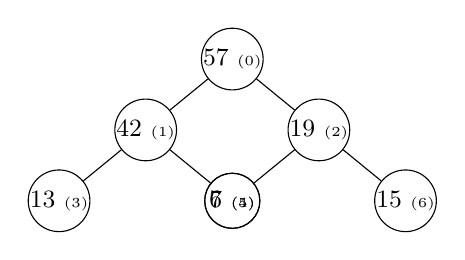
\begin{tikzpicture}[level distance=9mm, sibling distance=22mm,
    every node/.style={circle, draw, minimum size=7mm, inner sep=0pt, font=\small}]
    \node {57 \tiny(0)}
        child {node {42 \tiny(1)}
            child {node {13 \tiny(3)}}
            child {node {6 \tiny(4)}}
        }
        child {node {19 \tiny(2)}
            child {node {7 \tiny(5)}}
            child {node {15 \tiny(6)}}
        };
\end{tikzpicture}
\end{center}

stored as:
\begin{center}
\begin{tabular}{|c|c|c|c|c|c|c|c|}
\hline
Index & 0 & 1 & 2 & 3 & 4 & 5 & 6 \\
\hline
Value & 57 & 42 & 19 & 13 & 6 & 7 & 15 \\
\hline
\end{tabular}
\end{center}

Check: \texttt{parent(4) = (4-1)/2 = 1}, so parent of $6$ is $42$ -- correct. \texttt{leftChild(2) = 5}, so left child of $19$ is $7$ -- correct.

\begin{ideabox}
A \emph{complete} binary tree has no gaps, so every array slot corresponds to an actual node. That's why the index formulas work -- if the tree had missing internal nodes, you'd need sentinels or a different encoding. This is the crucial reason heap insert and remove are written to \emph{preserve completeness structurally first} and fix the heap-property violation second.
\end{ideabox}

\subsection*{Why arrays beat pointers here}

\begin{center}
\begin{tabular}{ll}
Pointer-based tree       & Array-based heap \\
\hline
3 pointers per node (24 B on 64-bit) & No per-element overhead \\
Cache miss per child jump           & Cache-friendly (children are 1--2 cells ahead) \\
\texttt{new}/\texttt{delete} per insert/remove & \texttt{vector} grows amortized $O(1)$ \\
Works for arbitrary tree shapes     & Requires completeness \\
\end{tabular}
\end{center}

For a heap of a million ints: pointer representation is $\approx 28$ MB of overhead beyond the values themselves; array representation is $\approx 0$ overhead. The array form is also a contiguous memory block, so sequential scans (like heapsort) are prefetch-friendly.

\subsection*{Percolate-up, array version}

Starting at some index \texttt{i} where the heap property might be broken upward, walk toward the root swapping with parent while the child is larger:

\begin{lstlisting}
void maxHeapPercolateUp(int i, std::vector<int>& h) {
    while (i > 0) {
        int parent = (i - 1) / 2;
        if (h[i] <= h[parent]) return;          // heap property satisfied
        std::swap(h[i], h[parent]);
        i = parent;                              // continue from new position
    }
}
\end{lstlisting}

The loop runs at most $\lfloor \log_2 n \rfloor$ times because each iteration halves the index. That's the $O(\log n)$ insert bound.

\subsection*{Percolate-down, array version}

Starting at some index \texttt{i} (usually 0, after the root was replaced), walk toward the leaves swapping with the larger child while a child is larger than the node:

\begin{lstlisting}
void maxHeapPercolateDown(int i, std::vector<int>& h) {
    int n = static_cast<int>(h.size());
    while (2 * i + 1 < n) {                      // at least one child exists
        int left  = 2 * i + 1;
        int right = 2 * i + 2;
        int biggest = left;
        if (right < n && h[right] > h[left]) biggest = right;
        if (h[i] >= h[biggest]) return;          // heap property satisfied
        std::swap(h[i], h[biggest]);
        i = biggest;
    }
}
\end{lstlisting}

Watch the three subtleties:
\begin{itemize}[leftmargin=*]
    \item \textbf{Check left first.} If \texttt{2*i+1 >= n}, \texttt{i} is a leaf and we're done.
    \item \textbf{Right might not exist.} That's why the right comparison is guarded by \texttt{right < n}.
    \item \textbf{Swap with the \emph{larger} child, not an arbitrary child.} If you swap with the smaller, the larger child becomes the new root and you've created a new violation below.
\end{itemize}

The loop runs at most $\lfloor \log_2 n \rfloor$ times (each iteration doubles the index). That's the $O(\log n)$ extract-max bound.

\begin{warnbox}
Off-by-one bugs are the dominant failure mode here. Triple-check your index formulas -- $(i-1)/2$ for parent uses integer division, which works because the formula is exact for both left ($i = 2p+1$) and right ($i = 2p+2$) children. Writing $i/2 - 1$ or $i/2$ will pass for some inputs and silently corrupt for others.
\end{warnbox}

\subsection*{Insert and extract, array versions}

\begin{lstlisting}
void maxHeapInsert(std::vector<int>& h, int value) {
    h.push_back(value);                          // step 1: preserve completeness
    maxHeapPercolateUp(h.size() - 1, h);         // step 2: restore heap property
}

int maxHeapExtract(std::vector<int>& h) {
    int top = h[0];
    h[0] = h.back();                             // move last to root
    h.pop_back();                                // shrink
    if (!h.empty()) maxHeapPercolateDown(0, h);
    return top;
}
\end{lstlisting}

Two functions, each $O(\log n)$ worst case, each three lines of logic. No tree allocations, no node structs, no parent pointers. The index formulas are the whole trick.

\begin{notebox}
\textbf{Zero-indexed vs.\ one-indexed.} Some textbooks and papers use index 1 as the root and leave index 0 unused. Then $\text{parent}(i) = i/2$, $\text{left}(i) = 2i$, $\text{right}(i) = 2i + 1$ -- slightly cleaner math. C++ code defaults to zero-indexed because \texttt{std::vector} is zero-indexed. Don't mix conventions in one codebase; pick one and stick with it. This course uses zero-indexed.
\end{notebox}

\section{7.3 Heapsort}

Heapsort is the sorting algorithm you get almost for free once you have a heap. The idea: turn an array into a max-heap, then repeatedly extract the max to the end of the array. You end up with an array sorted in ascending order, using \emph{no extra memory beyond the input array itself}.

Two phases:
\begin{enumerate}[leftmargin=*]
    \item \textbf{Heapify} the input array in place -- transform it into a valid max-heap.
    \item \textbf{Sort down}: swap \texttt{arr[0]} (the max) with the last unsorted slot, shrink the heap by one, and percolate the new root down. Repeat until the heap is empty.
\end{enumerate}

Both phases use one primitive: \texttt{maxHeapPercolateDown} from section 7.2.

\subsection*{Heapify: bottom-up heap construction}

Given an arbitrary array, how do we make it a max-heap? Naive approach: insert all elements one by one, each an $O(\log n)$ operation -- total $O(n \log n)$. There is a better way.

\begin{defnbox}[Heapify]
Call \texttt{percolateDown} on every internal node in reverse index order, from the last internal node down to the root. Leaves are trivially heaps (no children to violate anything), and each percolate-down restores the heap property over its subtree assuming the children are already valid heaps.
\end{defnbox}

The last internal node is at index $\lfloor n/2 \rfloor - 1$, because nodes at index $\ge \lfloor n/2 \rfloor$ are leaves (their first child index $2i + 1$ is out of range).

\begin{lstlisting}
void heapify(std::vector<int>& a) {
    for (int i = static_cast<int>(a.size()) / 2 - 1; i >= 0; --i)
        maxHeapPercolateDown(i, a);
}
\end{lstlisting}

\subsection*{Why heapify is $O(n)$, not $O(n \log n)$}

This is the cleverness of bottom-up construction, and it catches most students off-guard on exams.

Percolate-down at index $i$ does work proportional to the \emph{height of the subtree rooted at $i$}, not the total height of the tree. A leaf has height 0 (does no work). A parent of leaves has height 1 (at most 1 swap). The root has height $\log n$. Summed over all nodes:

\[
\sum_{i=0}^{\lfloor \log n \rfloor} (\text{nodes at height } i) \cdot i
= \sum_{i=0}^{\lfloor \log n \rfloor} \frac{n}{2^{i+1}} \cdot i
= O(n)
\]

The geometric series in $i/2^i$ converges to a constant. Half the nodes are leaves (do 0 work), a quarter do at most 1 swap, an eighth do at most 2 swaps, and so on. The totals balance out to $O(n)$.

\begin{ideabox}
This is the right mental image: bottom-up heapify cheats the worst case because \emph{most of the nodes are near the bottom where their percolate-down has nothing to do.} Repeated insertion is $O(n \log n)$ because it forces every element through a full height's worth of potential swaps. Same final data structure, different total cost. Prefer heapify over ``insert one by one'' whenever you have all the data up front.
\end{ideabox}

\subsection*{The sort-down phase}

After heapify, \texttt{a[0]} holds the maximum. The classic ``swap with last, shrink heap, percolate down'' trick used in \texttt{maxHeapExtract} (section 7.2) -- but we keep the extracted value in the array instead of returning it:

\begin{lstlisting}
void heapSort(std::vector<int>& a) {
    heapify(a);

    int n = static_cast<int>(a.size());
    for (int end = n - 1; end > 0; --end) {
        std::swap(a[0], a[end]);            // move current max to its final spot
        maxHeapPercolateDown(0, a, end);    // heap is now indices [0, end)
    }
}
\end{lstlisting}

Notice the overloaded \texttt{percolateDown} here takes an explicit \texttt{size} parameter -- after each swap, the last slot is ``sorted off'' and the heap shrinks. You're not physically removing elements; you're just treating the suffix as already-sorted.

\subsection*{Walk-through}

Sort \texttt{[11, 21, 12, 13, 19, 15]}.

Step 1 -- heapify, starting at index $\lfloor 6/2 \rfloor - 1 = 2$:

\begin{center}
\begin{tabular}{lllllll}
Before: & 11 & 21 & 12 & 13 & 19 & 15 \\
percolateDown(2): node 12 vs children (15) -- swap 12, 15 \\
 & 11 & 21 & \textbf{15} & 13 & 19 & \textbf{12} \\
percolateDown(1): node 21 vs children (13, 19) -- already biggest \\
 & 11 & 21 & 15 & 13 & 19 & 12 \\
percolateDown(0): node 11 vs (21, 15) -- swap with 21; then 11 vs (13, 19) -- swap with 19 \\
 & \textbf{21} & \textbf{19} & 15 & 13 & \textbf{11} & 12 \\
\end{tabular}
\end{center}

Step 2 -- sort down:

\begin{center}
\begin{tabular}{llllllll}
 & 21 & 19 & 15 & 13 & 11 & 12 \\
swap a[0]=21, a[5]=12; heap size 5; percolate 12 $\to$ children (19, 15) swap 12,19; then (13,11) stay \\
 & 19 & 13 & 15 & 12 & 11 & \textbf{21} \\
swap a[0]=19, a[4]=11; size 4; percolate 11 $\to$ (13, 15) swap 11, 15; then (12) stay \\
 & 15 & 13 & 11 & 12 & \textbf{19} & 21 \\
swap a[0]=15, a[3]=12; size 3; percolate 12 $\to$ (13, 11) swap 12, 13 \\
 & 13 & 12 & 11 & \textbf{15} & 19 & 21 \\
swap a[0]=13, a[2]=11; size 2; percolate 11 $\to$ (12) swap \\
 & 12 & 11 & \textbf{13} & 15 & 19 & 21 \\
swap a[0]=12, a[1]=11; size 1; done \\
 & 11 & \textbf{12} & 13 & 15 & 19 & 21 \\
\end{tabular}
\end{center}

Final: \texttt{[11, 12, 13, 15, 19, 21]}. Sorted ascending.

\subsection*{Cost analysis}

\begin{center}
\begin{tabular}{lll}
Phase & Per step & Total \\
\hline
Heapify              & up to $O(\log n)$ per node & $O(n)$ total (the geometric sum) \\
Sort-down            & $O(\log n)$ per extraction & $O(n \log n)$ \\
\hline
\textbf{Heapsort}    & & $\mathbf{O(n \log n)}$ \\
\end{tabular}
\end{center}

Space: $O(1)$ auxiliary. Heapsort is the canonical \emph{in-place} $O(n \log n)$ sort -- it rearranges the input array without needing a second array.

\subsection*{Heapsort vs.\ quicksort vs.\ mergesort}

\begin{center}
\begin{tabular}{llll}
Algorithm & Worst case & Space & Stable? \\
\hline
Quicksort   & $O(n^2)$      & $O(\log n)$ stack & no \\
Mergesort   & $O(n \log n)$ & $O(n)$            & yes \\
Heapsort    & $O(n \log n)$ & $O(1)$            & no \\
\end{tabular}
\end{center}

Heapsort's killer feature is the combination of $O(n \log n)$ \emph{worst case} and $O(1)$ auxiliary space. Quicksort has a worst case of $O(n^2)$; mergesort needs $O(n)$ extra memory. In practice, quicksort is usually fastest due to cache effects, but heapsort is picked when you need worst-case guarantees (embedded systems, real-time deadlines, adversarial inputs).

\begin{warnbox}
Heapsort is \textbf{not stable}: equal keys may swap order during the percolate steps. If stability matters (sorting records by one field without disturbing existing order on another), use mergesort or a stable quicksort variant, not heapsort.
\end{warnbox}

\begin{notebox}
\texttt{std::sort\_heap} and \texttt{std::make\_heap} in \texttt{<algorithm>} give you the two phases of heapsort. \texttt{std::partial\_sort} uses a heap-based algorithm to find and sort the top $k$ in $O(n \log k)$. None of these are the full \texttt{std::sort}, which typically uses introsort (quicksort that falls back to heapsort when recursion depth gets bad) -- precisely because heapsort's worst-case guarantee is the backup plan when quicksort starts to degrade.
\end{notebox}

\section{7.4 The Priority Queue ADT}

Section 7.1 motivated heaps with the priority-queue use case. This section formalizes the \emph{abstract data type} (ADT) and shows why heaps are the near-universal implementation. An ADT is a specification of operations and their contracts -- it tells you \emph{what} a data structure does, not \emph{how} it's implemented.

\begin{defnbox}[Priority queue]
A \textbf{priority queue} (PQ) is a collection where each element has a priority. The defining operations:
\begin{itemize}[leftmargin=*]
    \item \texttt{push(item)} -- insert an element.
    \item \texttt{pop()} -- remove and return the highest-priority element.
    \item \texttt{peek()} -- return (but don't remove) the highest-priority element.
    \item \texttt{isEmpty()} / \texttt{size()} -- the obvious.
\end{itemize}
``Highest priority'' can mean max-key or min-key depending on whether you want a max-PQ or min-PQ.
\end{defnbox}

Notice what the ADT \emph{doesn't} promise: arbitrary search, ordered iteration, range queries, positional access. A priority queue is FIFO ordered only among items of equal priority (that's the ``queue'' part), and even that is often not guaranteed unless the implementation makes a point of preserving it.

\subsection*{Two conventions for ``priority''}

A priority queue implementation has to answer: does the caller supply a priority alongside each item, or does the item carry its own priority?

\textbf{Separate-priority API:}

\begin{lstlisting}
pq.pushWithPriority(jobPointer, priorityNumber);
auto best = pq.pop();   // returns the stored item (not the priority)
\end{lstlisting}

Natural when the same object might live in multiple PQs with different priorities (e.g., a process could be in a CPU scheduler keyed by niceness and in an I/O scheduler keyed by deadline).

\textbf{Self-priority API:}

\begin{lstlisting}
struct Customer { std::string name; int waitScore; };
// ordering comparator compares on waitScore
pq.push(customer);
auto next = pq.pop();
\end{lstlisting}

Natural when priority is a property of the item itself. This is what \texttt{std::priority\_queue} does -- it takes a comparator and compares items directly.

Both are just different ways to express the same underlying concept. The self-priority API typically requires a comparator; the separate-priority API stores \texttt{(priority, item)} pairs and compares on the first component.

\subsection*{Contract summary}

\begin{center}
\begin{tabular}{lll}
Operation & Pre-condition & Post-condition \\
\hline
\texttt{push(x)}     & heap has room (or is resizable) & $x$ is in the PQ; size $+1$ \\
\texttt{pop()}       & PQ is non-empty & returns the max/min; that item is removed; size $-1$ \\
\texttt{peek()}      & PQ is non-empty & returns the max/min; PQ unchanged \\
\texttt{isEmpty()}   & none & true iff size $= 0$ \\
\texttt{size()}      & none & returns non-negative count \\
\end{tabular}
\end{center}

Violating the pre-condition (\texttt{pop} on empty) is undefined behavior in C++'s \texttt{std::priority\_queue}; Java's \texttt{PriorityQueue} returns null or throws \texttt{NoSuchElementException} depending on which method you call (\texttt{poll} vs.\ \texttt{remove}). Always check \texttt{isEmpty()} first, or wrap the call in a try/check.

\subsection*{Why heaps are the default implementation}

\begin{center}
\begin{tabular}{lllll}
Backing structure & push & pop (max) & peek & extra notes \\
\hline
Unsorted array/list   & $O(1)$      & $O(n)$     & $O(n)$ & peek rescans \\
Sorted array          & $O(n)$      & $O(1)$     & $O(1)$ & insert shifts \\
Sorted linked list    & $O(n)$      & $O(1)$     & $O(1)$ & insert scans \\
Balanced BST          & $O(\log n)$ & $O(\log n)$ & $O(\log n)$ & overkill, higher constants \\
\textbf{Binary heap}  & $O(\log n)$ & $O(\log n)$ & $O(1)$  & tight constants, cache-friendly \\
Fibonacci heap        & $O(1)$ amort. & $O(\log n)$ amort. & $O(1)$ & complex, big constants \\
\end{tabular}
\end{center}

The binary heap is the \emph{simplest} structure that gives log-factor bounds on both push and pop with $O(1)$ peek. It's also the one where the implementation is small, cache-friendly, and easy to reason about. Fibonacci heaps have better asymptotic bounds but their constant factors are so bad they're only a win at sizes real problems don't usually reach.

\subsection*{Mapping PQ operations to heap operations}

\begin{center}
\begin{tabular}{lll}
PQ op & Heap op (section 7.2) & Cost \\
\hline
\texttt{push(x)}   & \texttt{maxHeapInsert}: push to back, percolate up & $O(\log n)$ \\
\texttt{pop()}     & \texttt{maxHeapExtract}: swap root/last, pop, percolate down & $O(\log n)$ \\
\texttt{peek()}    & return \texttt{h[0]} & $O(1)$ \\
\texttt{isEmpty()} & return \texttt{h.empty()} & $O(1)$ \\
\texttt{size()}    & return \texttt{h.size()} & $O(1)$ \\
\end{tabular}
\end{center}

A priority queue is, in essentially all real codebases, just a thin wrapper around a heap's array.

\subsection*{Implementation sketch in C++}

\begin{lstlisting}
template <typename T, typename Cmp = std::less<T>>
class PriorityQueue {
    std::vector<T> h_;
    Cmp cmp_;   // cmp_(a, b) == true means "a has lower priority than b"
                // For a max-heap with std::less, cmp_(a, b) is a < b,
                // which is what we percolate up on.

    void percolateUp(std::size_t i) {
        while (i > 0) {
            std::size_t p = (i - 1) / 2;
            if (!cmp_(h_[p], h_[i])) return;        // parent is larger already
            std::swap(h_[p], h_[i]);
            i = p;
        }
    }
    void percolateDown(std::size_t i) {
        std::size_t n = h_.size();
        while (2 * i + 1 < n) {
            std::size_t l = 2 * i + 1, r = 2 * i + 2, best = l;
            if (r < n && cmp_(h_[l], h_[r])) best = r;
            if (!cmp_(h_[i], h_[best])) return;
            std::swap(h_[i], h_[best]);
            i = best;
        }
    }
public:
    bool empty() const { return h_.empty(); }
    std::size_t size() const { return h_.size(); }
    const T& peek() const { return h_.front(); }

    void push(T value) {
        h_.push_back(std::move(value));
        percolateUp(h_.size() - 1);
    }
    T pop() {
        T top = std::move(h_.front());
        h_.front() = std::move(h_.back());
        h_.pop_back();
        if (!h_.empty()) percolateDown(0);
        return top;
    }
};
\end{lstlisting}

That's 40 lines for a complete priority queue. The \texttt{std::priority\_queue} in the standard library is essentially this, with a few more template knobs.

\subsection*{Using \texttt{std::priority\_queue}}

\begin{lstlisting}
#include <queue>
#include <vector>

// Max-heap of ints
std::priority_queue<int> maxPQ;
maxPQ.push(5); maxPQ.push(1); maxPQ.push(9);
maxPQ.top();   // 9
maxPQ.pop();
maxPQ.top();   // 5

// Min-heap of ints
std::priority_queue<int, std::vector<int>, std::greater<int>> minPQ;

// Custom comparator on (priority, payload) pairs
using Entry = std::pair<int, std::string>;
auto cmp = [](const Entry& a, const Entry& b) { return a.first > b.first; };
std::priority_queue<Entry, std::vector<Entry>, decltype(cmp)> jobs(cmp);
jobs.push({3, "cleanup"}); jobs.push({1, "urgent"});
jobs.top();   // {1, "urgent"}   -- lower numeric priority = more urgent
\end{lstlisting}

\begin{warnbox}
\texttt{std::priority\_queue::top} returns a \emph{const reference}. You cannot mutate the top element in place -- attempting to \texttt{const\_cast} it and rewrite would break the heap invariant. If you need to change a priority, you have to \texttt{pop} the item and \texttt{push} a new one, or switch to a structure with an \texttt{increase\_key} / \texttt{decrease\_key} operation (indexed heap, \texttt{std::multiset}, or a hand-written heap with a side-index).
\end{warnbox}

\begin{ideabox}
An ADT separates ``what a structure promises'' from ``how it does it.'' Everywhere in this course, when a problem reduces to ``I keep needing the extremum of a changing set,'' you should reach for a priority queue -- and under the hood, you can bet it's a heap.
\end{ideabox}

\section{7.5 Treaps: Heap + BST}

Chapter 6 ended with a warning: a raw BST collapses on sorted input. Chapter 6.10 teased self-balancing trees (AVL, red-black) as the rigorous fix. This section shows a \emph{lazier} fix -- a fix that doesn't require tracking balance factors or recoloring -- called a \textbf{treap} (tree + heap).

\begin{defnbox}[Treap]
A treap is a binary tree where each node carries two keys:
\begin{itemize}[leftmargin=*]
    \item A \textbf{main key} (the data you care about), maintained in \emph{BST order} across the tree.
    \item A \textbf{priority} (a random number chosen when the node is inserted), maintained in \emph{heap order} across the tree.
\end{itemize}
Both invariants hold simultaneously: for every node $n$, main-keys follow the BST rule w.r.t.\ subtrees, and priorities follow the heap rule w.r.t.\ parent/child.
\end{defnbox}

The magic observation: \emph{given a set of (main key, priority) pairs with distinct priorities, there is exactly one tree shape that satisfies both invariants.} The highest-priority node has to be the root (heap), and among its descendants the BST ordering is determined. So if priorities are random, the tree's shape is the same tree you'd get by inserting the main keys in the \emph{random order of their priorities}. And we already know: random-order BST insertion gives expected $O(\log n)$ height.

The treap is a self-balancing BST that achieves expected $O(\log n)$ operations by \emph{randomizing its insertion order internally}, without the caller having to cooperate.

\subsection*{The missing primitive: rotations}

Percolate-up in a normal heap swaps parent and child. That breaks the BST ordering. Treaps need a swap-like operation that \emph{preserves BST ordering}. That operation is the \textbf{rotation}, the same move AVL and red-black trees use.

\begin{defnbox}[Right rotation]
If $y$ is a node with left child $x$, right-rotating at $y$ makes $x$ the new root of the subtree, $y$ becomes $x$'s right child, and $x$'s former right child $B$ becomes $y$'s new left child. Left rotation is the mirror image.
\end{defnbox}

\begin{center}
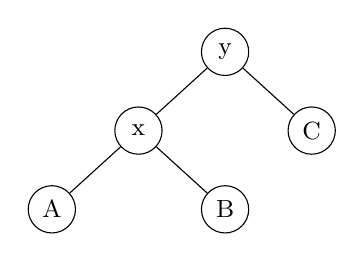
\begin{tikzpicture}[level distance=10mm, sibling distance=22mm,
    every node/.style={circle, draw, minimum size=6mm, inner sep=0pt, font=\small}]
    \node {y}
        child {node {x}
            child {node {A}}
            child {node {B}}
        }
        child {node {C}};
\end{tikzpicture}
\quad $\xrightarrow{\text{rotate right at } y}$ \quad
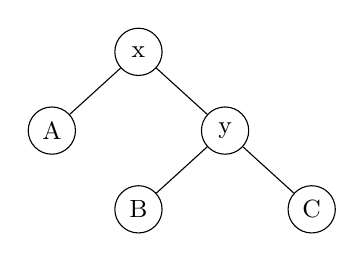
\begin{tikzpicture}[level distance=10mm, sibling distance=22mm,
    every node/.style={circle, draw, minimum size=6mm, inner sep=0pt, font=\small}]
    \node {x}
        child {node {A}}
        child {node {y}
            child {node {B}}
            child {node {C}}
        };
\end{tikzpicture}
\end{center}

Check ordering: before, $A < x < B < y < C$. After, still $A < x < B < y < C$. The in-order sequence is preserved. \emph{Heights and parent/child relationships change; BST ordering does not.}

Rotations are the universal self-balancing primitive. Once you have them, AVL, red-black, and treaps are all ``use rotations to restore some auxiliary invariant after a modification.'' The auxiliary invariant differs per structure; the mechanics are identical.

\subsection*{Treap insert}

\begin{enumerate}[leftmargin=*]
    \item Insert the new node at the right leaf position by main-key (pure BST insert).
    \item Assign it a random priority.
    \item While its priority exceeds its parent's priority, rotate so that the node moves up one level. \emph{Rotate right} if the node is a left child; \emph{rotate left} if it is a right child.
\end{enumerate}

The rotation choice is forced: to move a left-child upward, only a right-rotation at the parent works; analogously for a right-child and left-rotation. Each rotation preserves BST ordering and fixes one heap-property violation. After $O(\log n)$ expected rotations, the heap invariant is restored everywhere.

Example: start with a treap and insert key $B$ (assigned priority 70):

\begin{center}
\emph{After BST insert of B, before rotations:}
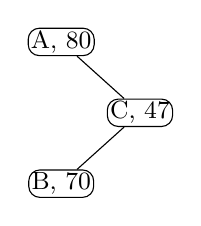
\begin{tikzpicture}[level distance=9mm, sibling distance=20mm,
    every node/.style={rectangle, draw, rounded corners, inner sep=1pt, font=\small}]
    \node {A, 80}
        child[missing] {}
        child {node {C, 47}
            child {node {B, 70}} child[missing] {}
        };
\end{tikzpicture}
\end{center}

Heap violation: parent \texttt{C}'s priority 47 is less than \texttt{B}'s 70. \texttt{B} is a left child, so rotate right at \texttt{C}:

\begin{center}
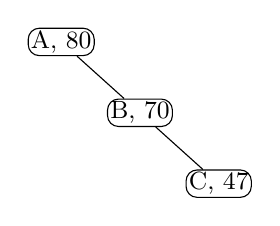
\begin{tikzpicture}[level distance=9mm, sibling distance=20mm,
    every node/.style={rectangle, draw, rounded corners, inner sep=1pt, font=\small}]
    \node {A, 80}
        child[missing] {}
        child {node {B, 70}
            child[missing] {}
            child {node {C, 47}}
        };
\end{tikzpicture}
\end{center}

Now \texttt{B}'s parent is \texttt{A} with priority 80 -- heap holds (80 $>$ 70). Stop. Treap restored.

\subsection*{Treap delete}

To delete a node $X$:
\begin{enumerate}[leftmargin=*]
    \item Pretend $X$'s priority is $-\infty$ (lowest possible). Now the heap property is violated at $X$: every child's priority is greater.
    \item Percolate $X$ down by rotating it with the \emph{higher-priority} child. That child becomes the new subtree root, $X$ sinks one level. Continue until $X$ has no children.
    \item Unhook and delete $X$.
\end{enumerate}

The ``higher-priority child'' rule matters: rotating with the \emph{lower}-priority child would leave a new heap violation in place of the old one. Rotating with the higher-priority child lifts it up and fixes the violation at that level.

Example: delete node \texttt{F} from a tree where its children are \texttt{C} (priority 29) and \texttt{I} (priority 13). Assign \texttt{F}'s priority to $-\infty$. Higher-priority child is \texttt{C}, so rotate right at \texttt{F} (moving \texttt{C} up). Continue until \texttt{F} has no children, then delete.

\subsection*{Cost analysis}

All treap operations have \textbf{expected} cost $O(\log n)$, because the tree shape is (in expectation) the shape of a BST built from $n$ items inserted in random order -- expected height $O(\log n)$.

\begin{center}
\begin{tabular}{lll}
Operation & Expected & Worst-case \\
\hline
Search & $O(\log n)$ & $O(n)$ \\
Insert & $O(\log n)$ & $O(n)$ \\
Delete & $O(\log n)$ & $O(n)$ \\
\end{tabular}
\end{center}

The worst case is still $O(n)$ -- if your random-number generator has really bad luck, you could get a skewed tree. But the probability of this is exponentially small, so in practice treaps perform as well as AVL or red-black trees while being substantially simpler to implement.

\begin{ideabox}
A treap doesn't guarantee balance -- it \emph{randomizes} to make imbalance improbable. This is a common pattern in computer science: don't solve the hard version (guaranteed balance, as in AVL / red-black); randomize the input to dodge worst cases (as in quicksort, hash-function-seeded hash tables, skip lists, treaps). When randomization is acceptable, it's almost always easier to implement than the deterministic version.
\end{ideabox}

\subsection*{Treaps vs.\ AVL vs.\ red-black}

\begin{center}
\begin{tabular}{llll}
Structure & Balance guarantee & Implementation complexity & Used by \\
\hline
AVL         & strict $O(\log n)$           & medium   & older DB indexes \\
Red-black   & $O(\log n)$ (weaker balance) & high     & \texttt{std::map}, Linux kernel \\
Treap       & expected $O(\log n)$         & \textbf{low} & competitive programming, teaching \\
Skip list   & expected $O(\log n)$         & low       & Redis, LevelDB \\
\end{tabular}
\end{center}

Treaps are rarely the choice in production standard libraries (AVL and red-black trees' deterministic guarantees matter for adversarial workloads), but they're popular in competitive-programming circles for their tiny implementation. Roughly 30 lines of C++ gets you a working treap; a working red-black tree is 10$\times$ that.

\begin{notebox}
The trick of ``attach a random secondary key and let it drive structure'' is deeply generalizable. Skip lists use it for levels (each node has a random ``tower height''). Probabilistic data structures in databases (HyperLogLog, Count-Min sketches) use it for bucket assignments. Treaps are a clean, easy-to-visualize introduction to the technique.
\end{notebox}

\end{document}
